\documentclass[twocolumn, 9pt]{article}

\usepackage[margin=0.8in,bottom=1.25in,columnsep=.4in]{geometry}
\usepackage{amsmath}
\usepackage{amssymb}
\usepackage{listings}
\usepackage{color}
\usepackage{cite}
\usepackage{multicol}
\usepackage{booktabs}
\usepackage{graphicx}

\definecolor{codegreen}{rgb}{0,0.6,0}
\definecolor{codegray}{rgb}{0.5,0.5,0.5}
\definecolor{codepurple}{rgb}{0.58,0,0.82}
 
\lstdefinestyle{code}{
	% backgroundcolor=\color{bggray},
  commentstyle=\color{codegray},
  keywordstyle=\color{codegreen}\bfseries,
  stringstyle=\color{codepurple},
  basicstyle=\ttfamily\footnotesize,
  breakatwhitespace=false,     
  breaklines=true,         
  captionpos=b,          
  keepspaces=true,                  
  showspaces=false,        
  showstringspaces=false,
  showtabs=false,          
  tabsize=2
}
 
\lstset{style=code}

\title{
	50.039 Theory and Practice of Deep Learning\\
	Coding Homework 6
}

\author{Joel Huang 1002530}
\date{\today}

\begin{document}
\maketitle

\section{Accuracy on the test set}
I used a packed padded sequence input into a LSTM, followed by
a single fully-connected layer which accepts the LSTM's hidden
state as an output, reducing dimensionality to the number of classes.
Where the layer size is greater than 1, we have a stacked LSTM. Besides
concatenating the hidden states from all layers (which would require a
change in the dimensionality of the fully-connected layer), and averaging
across all hidden states, another option is to feed the top-most layer's
hidden state as it's a downstream output from the hidden states before it.

\begin{table}[h]
  \centering
  \begin{tabular}{lll}
    \toprule
    Hyperparameter    & Value  \\
    \midrule
    Epochs            & 20     \\
    Batch size        & 16     \\
    Optimizer         & Adam   \\
    Learning rate     & 1e-3   \\
    Loss weights      & None   \\
    Hidden dimensions & [32,64,128]\\
    LSTM layers       & [1,2]  \\
    \bottomrule
  \end{tabular}
  \caption{Hyperparameter selection for Task 1.}
  \label{tab:hyp1}
\end{table}

I used a 70:30 split for the training and test sets. The entire dataset
(of length 20k) is shuffled before splitting. Purely random sampling is
used in our training. We train with cross-entropy loss using the Adam
optimizer. The rest of the training hyperparameters are shown in
Table~\ref{tab:hyp1}.

\subsubsection*{Results}
Training batches of 16 over 20 epochs with no early stopping yields the
results as shown in Table~\ref{tab:res1}.
\begin{table}[h]
  \centering
  \begin{tabular}{llll}
    \toprule
    Number & Hidden & Test & Test \\
    of layers & size & loss & accuracy \\
    \midrule
    1 & 32  & 0.899 & 78.8 \\
    1 & 64  & 0.885 & 80.4 \\
    1 & 128 & 0.928 & 79.5 \\
    2 & 32  & 0.890 & 79.4 \\
    2 & 64  & 0.914 & 78.4 \\
    2 & 128 & 0.958 & 80.4 \\
    \bottomrule
  \end{tabular}
  \caption{Test results for Task 1.}
  \label{tab:res1}
\end{table}

\section{Batched LSTM}
LSTM can be run with batches but requires fixed-size sequences for each
sample in the batch. To deal with this, we first shortlist a mini-batch
of samples. The samples of varying sequence length are then zero-padded
to match the length of the longest sequence in the mini-batch. They are
then packed and fed into the LSTM.

\begin{table}[h]
  \centering
  \begin{tabular}{lll}
    \toprule
    Hyperparameter    & Value  \\
    \midrule
    Epochs            & 20     \\
    Batch size        & [1,10,30]\\
    Optimizer         & Adam   \\
    Learning rate     & 1e-3   \\
    Loss weights      & None   \\
    Hidden dimensions & 200    \\
    LSTM layers       & 1      \\
    \bottomrule
  \end{tabular}
  \caption{Hyperparameter selection for Task 2.}
  \label{tab:hyp2}
\end{table}

We'll compare the training and test error, and test accuracy for the
hyperparameter set in Table~\ref{tab:hyp2}, using a 70:10:20 split for
training, validation and test sets respectively, training for 20 epochs.

\subsubsection*{Results}

\begin{figure}[htbp]
	\centering
	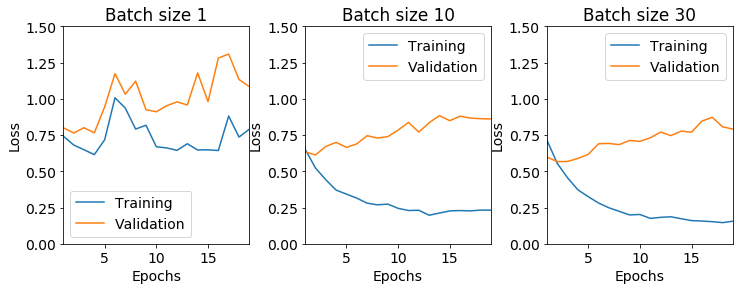
\includegraphics[width=\columnwidth]{lossacc.png}
	\caption{Individual training and validation losses for batch sizes 1, 10 and 30.}
	\label{fig:indiv}
\end{figure}

The individual plots of training vs. validation losses can be seen in Fig.~\ref{fig:indiv}.
Training with a batch size of 1 took extremely long and losses did not seem to converge
over 20 epochs. Training with a batch size of 10 and 30 resulted in losses converging,
with slight overfitting as seen in the plots.

\begin{figure}[htbp]
	\centering
	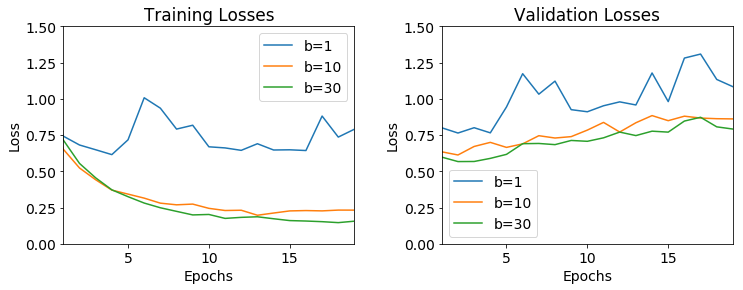
\includegraphics[width=\columnwidth]{valloss.png}
	\caption{Training and validation comparisons for batch sizes 1, 10 and 30.}
	\label{fig:compare}
\end{figure}

Comparing the training and validation losses with each other in Fig.~\ref{fig:compare},
we see the difference between batch size 1 and \{10, 30\} in greater contrast. Overall,
validation loss was increasing over 20 epochs almost right away after starting training,
while training loss converged for batch sizes \{10, 30\} but not for 1.

\begin{figure}[htbp]
	\centering
	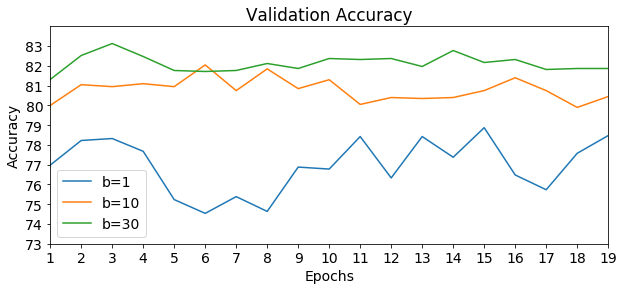
\includegraphics[width=\columnwidth]{valacc.png}
	\caption{Validation accuracy for batch sizes 1, 10 and 30.}
	\label{fig:acc}
\end{figure}

In Fig. ~\ref{fig:acc}, we see validation accuracy over the 20 epochs was fairly decent, with
clear differences. The higher the batch sizes, the greater the validation accuracy. We can
see a parallel result in Table ~\ref{tab:res2}, where performance (accuracy) on the test
set agrees with the validation accuracy banding.

\begin{table}[h]
  \centering
  \begin{tabular}{llll}
    \toprule
    Number & Hidden & Test & Test \\
    of layers & size & loss & accuracy \\
    \midrule
    1 & 200  & 1.137 & 76.8 \\
    1 & 200  & 0.902 & 80.1 \\
    1 & 200  & 0.847 & 81.3 \\
    \bottomrule
  \end{tabular}
  \caption{Test results for Task 2.}
  \label{tab:res2}
\end{table}

\section{Reproduction}
To reproduce the results, use the exact same dataset, with the hyperparameters used above.
Seed with \lstinline{torch.cuda.manual_seed_all(17)}, and a training set size of 14051,
validation set size of 2007, and test set size of 4016. I train with Python 3.7.2 on PyTorch
1.0.1.post2. Code is attached.
\end{document}